%%%%%%%%%%%%%%%%%%%%%%%
%% Folie             %%
%%%%%%%%%%%%%%%%%%%%%%%
\begin{frame}
    \frametitle{Reinforcement Learning (RL)}

Learns to solve tasks by maximizing the reward signal it gets
\vspace{10mm}

\begin{multicols}{2}
	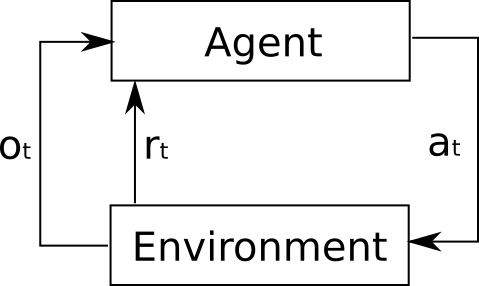
\includegraphics[width=0.9\columnwidth]{./Images/rl_agent.png}%
    \vfill\columnbreak	
	$a_i$: action\\
	$o_i$: observation\\
	$r_i$: reward
\end{multicols}

\end{frame}
\clearpage

%%%%%%%%%%%%%%%%%%%%%%%
%% Folie             %%
%%%%%%%%%%%%%%%%%%%%%%%
\begin{frame}
    \frametitle{Reinforcement Learning (RL)}

Model-free RL
\begin{PraesentationAufzaehlung}
	\item Observations of the environment map directly to values or actions	
\end{PraesentationAufzaehlung}
\vspace{-10mm}
Model-based RL
\begin{PraesentationAufzaehlung}
	\item Uses an internal model of the world to reason about the future
	\item Avoid adverse consequences of trial-and-error
	\item Increase performance by increasing amount of internal simulations
	%-- Better generalization across states%\\
\end{PraesentationAufzaehlung}

\end{frame}
\clearpage


%%%%%%%%%%%%%%%%%%%%%%%
%% Folie             %%
%%%%%%%%%%%%%%%%%%%%%%%
\begin{frame}
    \frametitle{Drawbacks of Model Based RL}


\begin{PraesentationAufzaehlung}
    \item The performance of model-based agents suffer if the model is inperfect\\
    \item It is not always possible to get an exact transition model
exact transition model is available
\end{PraesentationAufzaehlung}

$\rightarrow$ Combine model free and model based RL to get an agent\\
\hspace{8mm} which is robost against model imperfections.
\end{frame}
\clearpage


%%%%%%%%%%%%%%%%%%%%%%%
%% Folie             %%
%%%%%%%%%%%%%%%%%%%%%%%
\begin{frame}
    \frametitle{Advantage-Actor-Critic (A2C)}

Reinforcement Learning Algorithm
\begin{PraesentationAufzaehlung}
	\item Actor	learns policy function $\mathnormal{\pi(s, a, \theta)}$:\\
	Controls how the agent acts\\	
	\item Critic learns value function $\mathnormal{V(s, a, w)}$:\\
	Messures how good a choosen actions is\\
 	Expected cumulative reward from following the policy $\pi$ from state $s$	
\end{PraesentationAufzaehlung}



\end{frame}
\clearpage



%%%%%%%%%%%%%%%%%%%%%%%
%% Folie             %%
%%%%%%%%%%%%%%%%%%%%%%%
\begin{frame}
    \frametitle{Advantage-Actor-Critic (A2C)}

\begin{PraesentationAufzaehlung}
	\item Advantage function\\
		Push up the probability of an action from a state $s$ if this action was better than the expected value
		\begin{equation}
		\mathnormal{
		A = Q(s, a) - V(s)
%A^{\pi_\theta} = Q^{\pi_\theta}(s, a) - V^{\pi_\theta}(s)
		}
		\end{equation}
	\item Q-value function $Q(s, a)$:\\ %$Q^{\pi_\theta}(s, a)$:\\ 
		Expected cumulative reward from taking action $a$ in state $s$ and following the policy $\pi$
	\item Actor Critic policy update:
	\begin{equation}
		\mathnormal{
		\nabla \theta = A \nabla_\theta log \pi_\theta (a | s)}
	\end{equation}
\end{PraesentationAufzaehlung}

\end{frame}
\clearpage

%%%%%%%%%%%%%%%%%%%%%%%
%% Folie             %%
%%%%%%%%%%%%%%%%%%%%%%%
%\begin{frame}
%    \frametitle{Advantage-Actor-Critic (A2C)}

%\begin{PraesentationAufzaehlung}
%    \item Policy update:
%	\begin{equation}
%		\mathnormal{\nabla \theta = \alpha \nabla_\theta (log \pi_\theta (s, a)) q_w (s, a)}
%	\end{equation}	
%	\item Value update:
%	\begin{equation}
%		\mathnormal{
%		\nabla w = \beta (R(s, a) + \gamma q_w(s_{t+1}, a_{t+1}) - q_w(s_t, a_t)) \nabla_w q_w(s_t, a_t)}
%	\end{equation}
%\end{PraesentationAufzaehlung}

%\end{frame}
%\clearpage







%%%%%%%%%%%%%%%%%%%%%%%
%% Folie             %%
%%%%%%%%%%%%%%%%%%%%%%%
%\begin{frame}
%    \frametitle{What we want}

%\begin{multicols}{2}

%	Combine model free and model based RL to get an agent which is robost against model imperfections
%    \vfill\columnbreak
%	\begin{center}
%    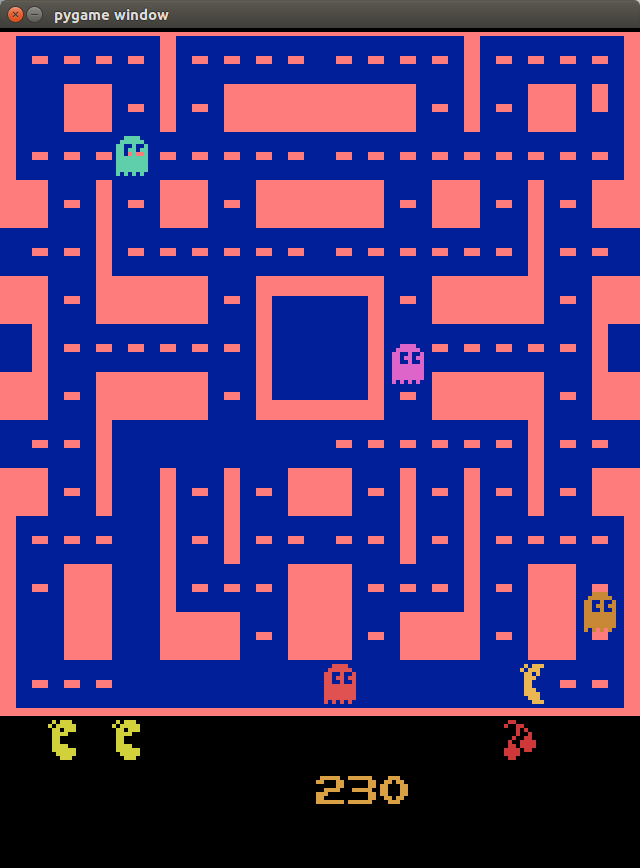
\includegraphics[height=.6\textheight]{./Images/screenshot_ghost.png}%
%	\end{center}
%\end{multicols}

	%We want an agent who learn to interpret predictions from a learned environment model to construct plans in arbitrary ways, by using the predictions as additional context in the deep policy network\\
%\end{frame}
%\clearpage



%%%%%%%%%%%%%%%%%%%%%%%
%% Folie             %%
%%%%%%%%%%%%%%%%%%%%%%%
%\begin{frame}
%    \frametitle{Goals}

%\begin{PraesentationAufzaehlung}
%    \item Working Implementation of I2A in pytorch
%\end{PraesentationAufzaehlung}

%\end{frame}
%\clearpage

%%%%%%%%%%%%%%%%%%%%%%%%%%%%%%%%%%%%%%%%%%%%%%%%%%%%%  
 % FOLIENSTIL: Weisse Schrift auf blauem Grund 
\PraesentationMasterWeissBlau 
\begin{frame} 
    \PraesentationUeberschriftZweizeilig{Imagination-Augmented Agent (I2A)}{Weber et al. (2017)}

\end{frame} 

\PraesentationMasterStandard


%%%%%%%%%%%%%%%%%%%%%%%
%% Folie             %%
%%%%%%%%%%%%%%%%%%%%%%%
\begin{frame}
    \frametitle{Imagination-Augmented Agent (I2A)}

\begin{PraesentationAufzaehlung}
	\item Weber et al.(2017)
    \item Imagine the future and learn to do better actions based on the imagined future
    \item Combines model-free and model-based aspects
\end{PraesentationAufzaehlung}

\end{frame}
\clearpage

%%%%%%%%%%%%%%%%%%%%%%%%%%%%%%%%%%%%%%%%
%% Folie: Bilder                      %%
%%%%%%%%%%%%%%%%%%%%%%%%%%%%%%%%%%%%%%%%
\begin{frame}
    \frametitle{I2A Architecture}


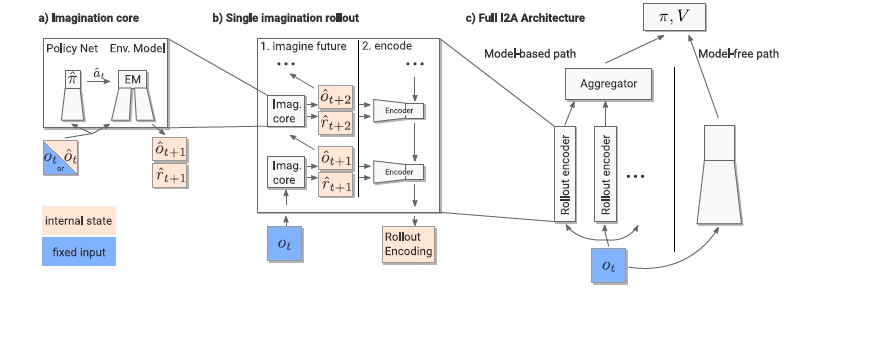
\includegraphics[width=\columnwidth]{./Images/i2a_architecture.png}%

\vspace{-10mm}
Network architecture for deep reinforcement learning which combines model free and model based RL

    
\end{frame}
\clearpage




%%%%%%%%%%%%%%%%%%%%%%%%%%%%%%%%%%%%%%%%
%% Folie: Bilder                      %%
%%%%%%%%%%%%%%%%%%%%%%%%%%%%%%%%%%%%%%%%
\begin{frame}
    \frametitle{Imagination Core}

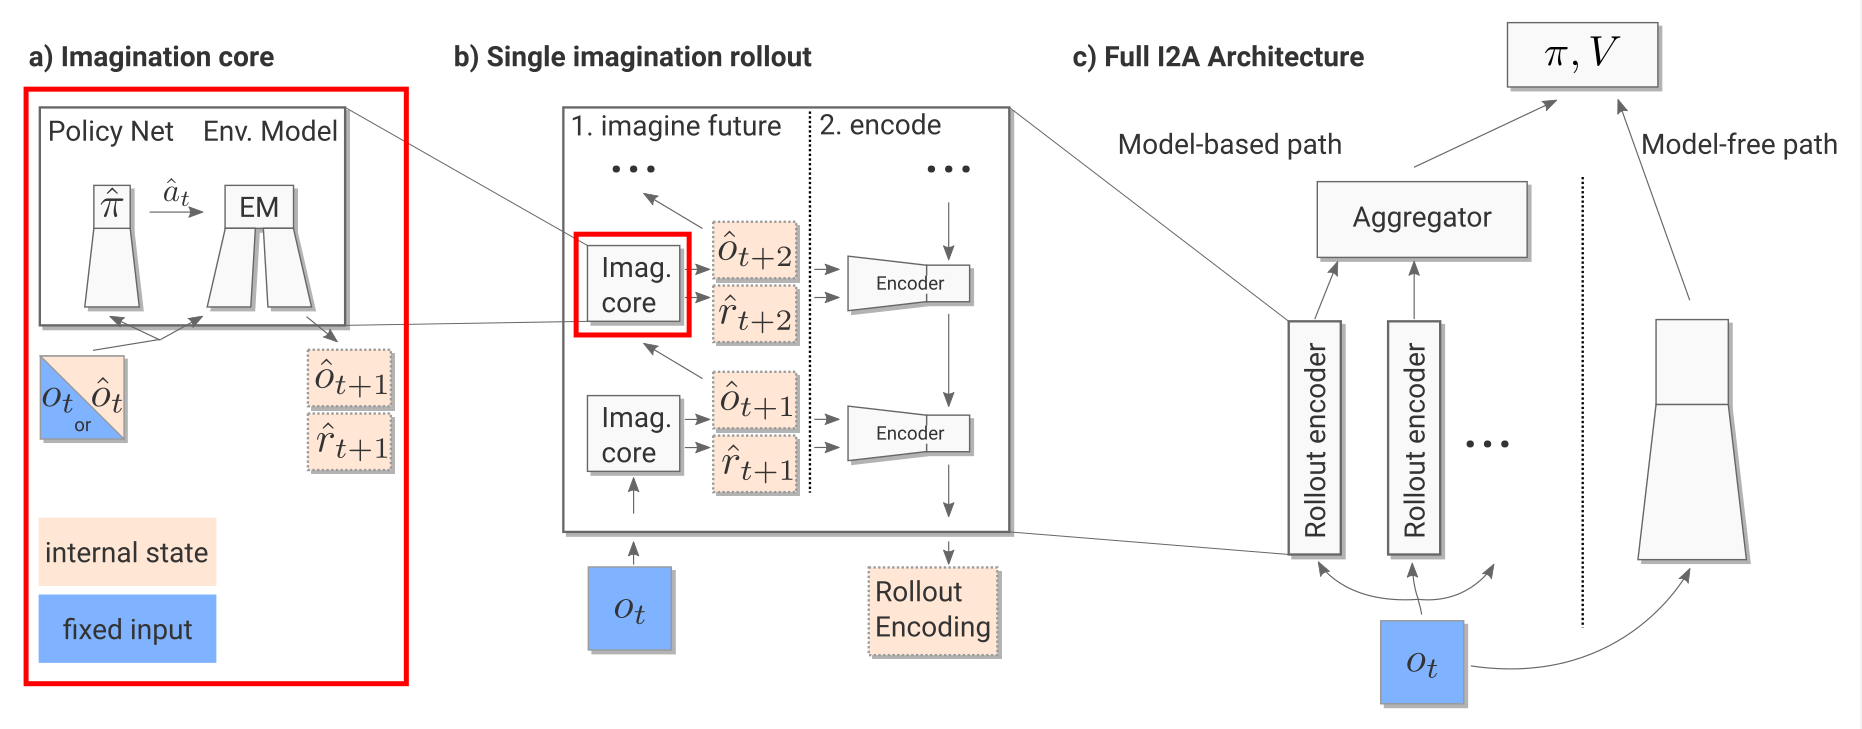
\includegraphics[width=\columnwidth]{./Images/i2a_all_imagination_core.png}%

\vspace{-10mm}
Imagine the next observation $\hat{o}_{t+i+1}$ and next reward $\hat{r}_{t+i+1}$ given observation $\hat{o}_{t+i}$ for n rollouts where $i = 0, ..., n$
%$\hat{}$
\end{frame}
\clearpage


%%%%%%%%%%%%%%%%%%%%%%%%%%%%%%%%%%%%%%%%
%% Folie: Bilder - Zweispaltige Seite %%
%%%%%%%%%%%%%%%%%%%%%%%%%%%%%%%%%%%%%%%%
%\begin{frame}
%    \frametitle{I2A Architecture - Imagination Core}

%\begin{multicols}{2}
%	\begin{PraesentationAufzaehlung}
%		\item Imaginate the next observation $o_{t+i}$ and next reward $r_{t+i}$ given observation $o_t$
%	\end{PraesentationAufzaehlung}
%    \vfill\columnbreak
%	\begin{center}
%    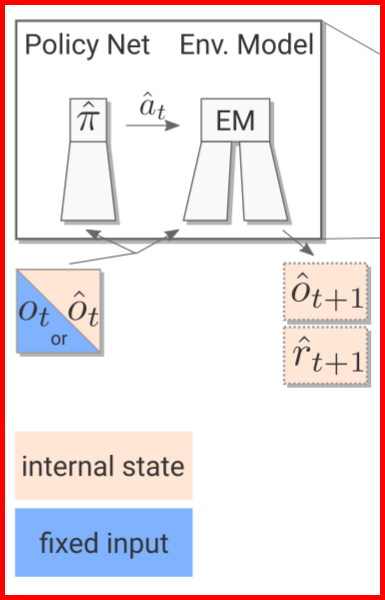
\includegraphics[height=0.5\textheight]{./Images/i2a_imagination_core.png}%
%	\end{center}
%\end{multicols}
    
%\end{frame}
%\clearpage

%%%%%%%%%%%%%%%%%%%%%%%%%%%%%%%%%%%%%%%%
%% Folie: Bilder - Zweispaltige Seite %%
%%%%%%%%%%%%%%%%%%%%%%%%%%%%%%%%%%%%%%%%
\begin{frame}
    \frametitle{Rollout Policy Network $\hat{\pi}$}

\begin{multicols}{2}
	\begin{PraesentationAufzaehlung}
	    \item Rollout policy network $\hat{\pi}$ decides the next action $\hat{a}_t$
		\item Distillation loss\\
		Make $\hat{\pi}$ (rollout policy) and $\pi$ (i2a policy) similar\\
	\end{PraesentationAufzaehlung}
    \vfill\columnbreak
	\begin{center}
    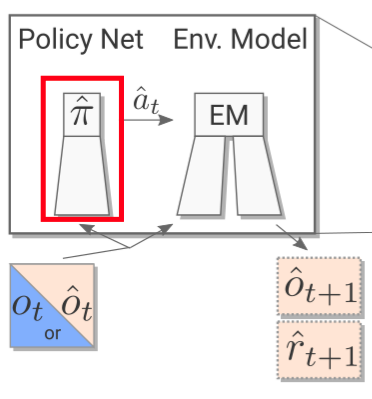
\includegraphics[height=0.35\textheight]{./Images/policy_net.png}%
	\end{center}
\end{multicols}
\vspace{-22mm}
\hspace{4mm}
Cross Entropy between $\pi$ and $\hat{\pi}$\\
	\begin{equation}
		\mathnormal{
		l_{dist}(\pi, \hat{\pi})(o_t) = \lambda_{dist} \sum_a \pi(a | o_t) log \hat{\pi}(a|o_t)
		}
	\end{equation}
    
\end{frame}
\clearpage


%%%%%%%%%%%%%%%%%%%%%%%%%%%%%%%%%%%%%%%%%%%%%%%%%%%%%  
 % FOLIENSTIL: Weisse Schrift auf blauem Grund 
%\PraesentationMasterWeissBlau 
%\begin{frame} 
%    \frametitle{Environment Model (EM)}
%\end{frame}

%\PraesentationMasterStandard

%%%%%%%%%%%%%%%%%%%%%%%%%%%%%%%%%%%%%%%%
%% Folie: Bilder - Zweispaltige Seite %%
%%%%%%%%%%%%%%%%%%%%%%%%%%%%%%%%%%%%%%%%
\begin{frame}
    \frametitle{Environment Model (EM)}

\begin{multicols}{2}
	\begin{PraesentationAufzaehlung}
	\item $o_t$: initial observation
	\item $\hat{o}_t$: predicted observation
	\item $\hat{r}_t$: predicted reward
		\item Given observation $o_t$ or $\hat{o}_t$ and action $\hat{a}_t$ predict (imagine) the next observation $\hat{o}_{t+1}$ and next reward $\hat{r}_{t+1}$ 
	\end{PraesentationAufzaehlung}
    \vfill\columnbreak
	\begin{center}
    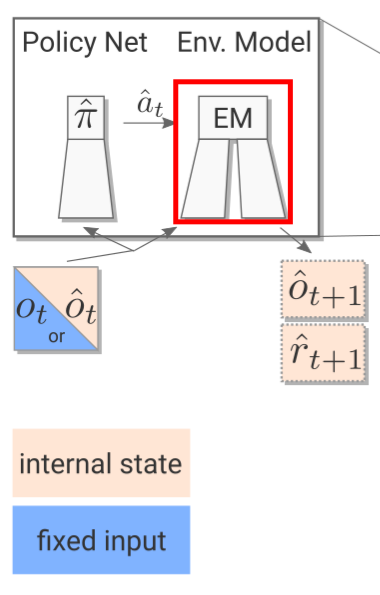
\includegraphics[height=0.5\textheight]{./Images/environment_model.png}%
	\end{center}
\end{multicols}
    
\end{frame}
\clearpage


%%%%%%%%%%%%%%%%%%%%%%%%%%%%%%%%%%%%%%%%
%% Folie: Bilder - Zweispaltige Seite %%
%%%%%%%%%%%%%%%%%%%%%%%%%%%%%%%%%%%%%%%%
\begin{frame}
    \frametitle{Environment Model Architecture}

\begin{multicols}{2}
	\begin{PraesentationAufzaehlung}
		\item Input:\\
		-- Stack of last 3 observations\\
		-- Action as one hot vector\\
		\item Trained with paris of $(o_t, a_t) \rightarrow (o_{t+1}, r_{t+1})$ generated from a pretrained model-free advantage-actor-critic policy
	\end{PraesentationAufzaehlung}
    \vfill\columnbreak
	\begin{center}
    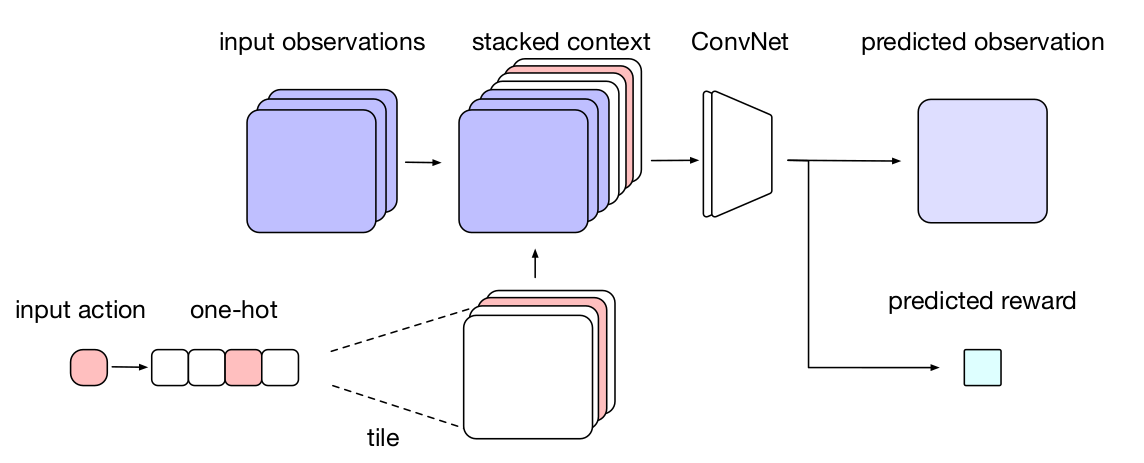
\includegraphics[width=\columnwidth]{./Images/environment_model_architecture.png}%
	\end{center}
\end{multicols}
    
\end{frame}
\clearpage




%%%%%%%%%%%%%%%%%%%%%%%%%%%%%%%%%%%%%%%%
%% Folie: Bilder - Zweispaltige Seite %%
%%%%%%%%%%%%%%%%%%%%%%%%%%%%%%%%%%%%%%%%
\begin{frame}
    \frametitle{Environment Model Training}

\begin{PraesentationAufzaehlung}
	\item Maximize the log likelihood of the probability $\mathnormal{p(o_t | a_{t-1}, o_{t-1})}$
	\item Image can be seen as Bernoulli distribution
	\begin{equation}
	\mathnormal{ p(o_t | a_{t-1}, o_{t-1}) = x^y (1-x)^{1-y}
	}
	\end{equation}
	\item  $\mathnormal{log p(o_t | a_{t-1}, o_{t-1})}$ equals to Binary Cross Entropy loss
	\begin{equation}
	\mathnormal{
	env_{loss}(x, y) = \frac{1}{N} \sum y_n log x_n + (1-y_n) log(1- x_n)
	%env_{loss} = Binary Cross Entropy(predicted\_image, true\_images)
	}
	\end{equation}
\end{PraesentationAufzaehlung}
    
\end{frame}
\clearpage



%%%%%%%%%%%%%%%%%%%%%%%%%%%%%%%%%%%%%%%%
%% Folie: Bilder                      %%
%%%%%%%%%%%%%%%%%%%%%%%%%%%%%%%%%%%%%%%%
\begin{frame}
    \frametitle{I2A Architecture - Imagination Rollout}


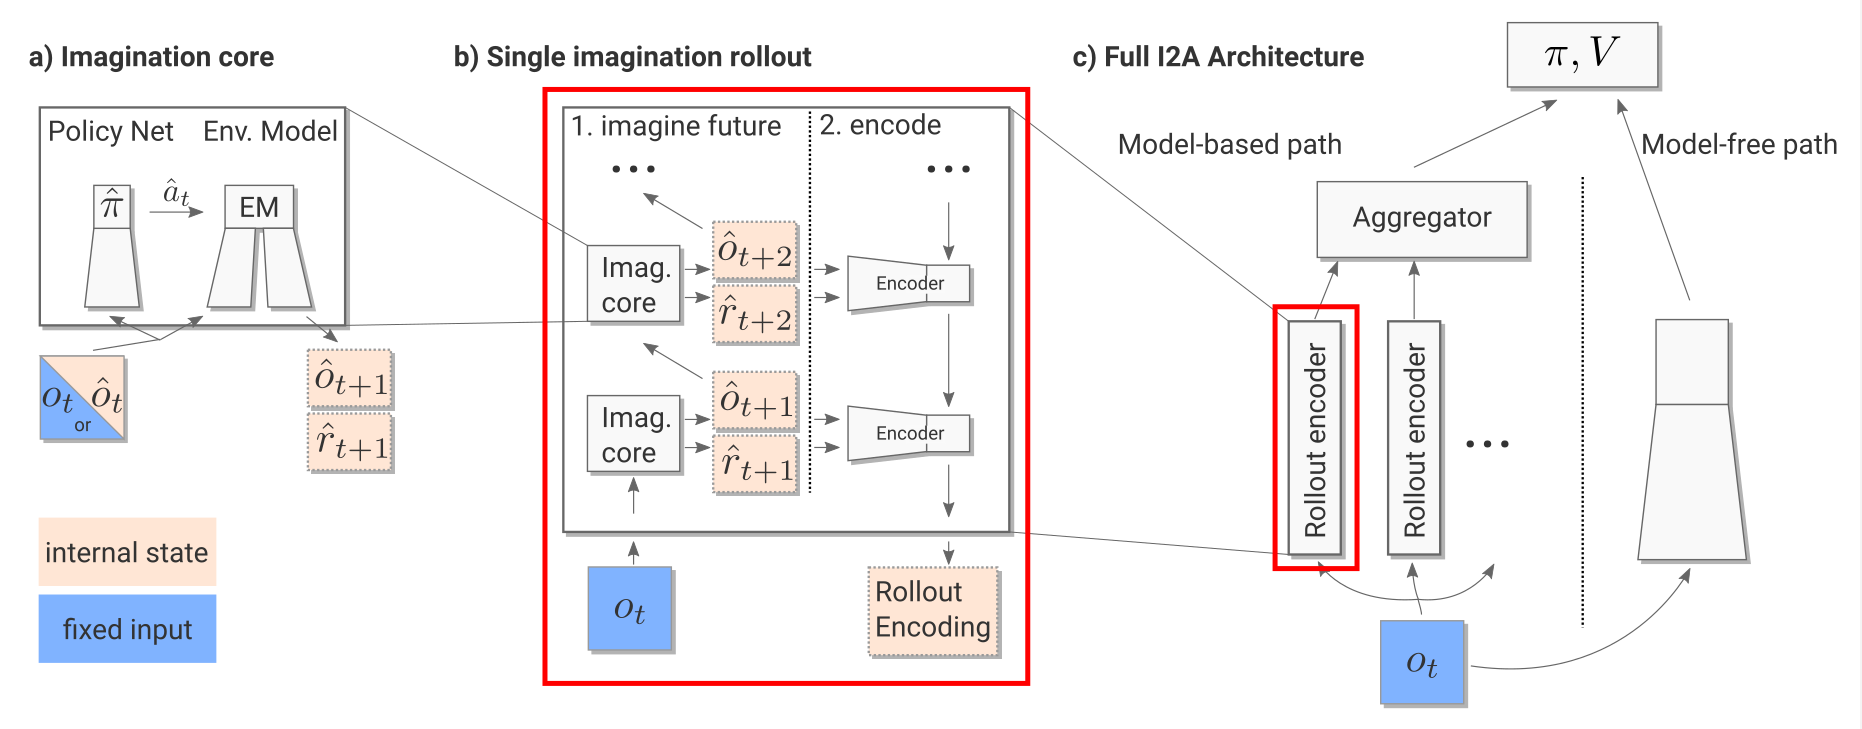
\includegraphics[width=\columnwidth]{./Images/i2a_all_imagination_rollout.png}%

\vspace{-10mm}
The imagination core imagines trajectories of features $f = (\hat{o}, \hat{r})$\\
The rollout encoder encode these trajectories    
\end{frame}
\clearpage


%%%%%%%%%%%%%%%%%%%%%%%%%%%%%%%%%%%%%%%%
%% Folie: Bilder - Zweispaltige Seite %%
%%%%%%%%%%%%%%%%%%%%%%%%%%%%%%%%%%%%%%%%
\begin{frame}
    \frametitle{I2A Architecture - Imagination Future}

\begin{multicols}{2}
	\begin{PraesentationAufzaehlung}
		\item Input:\\
		observation $o_t$ \\
		(1 MiniPacman frame)\\
		start action $a$
		\item Output:\\
		n imagined trajectories ($\hat{o}_{t+i}, \hat{r}_{t+i}$ for $i = 0, ..., n$)
		\item $\hat{} \hspace{2mm} \rightarrow$ internal state
	\end{PraesentationAufzaehlung}
    \vfill\columnbreak
	\begin{center}
    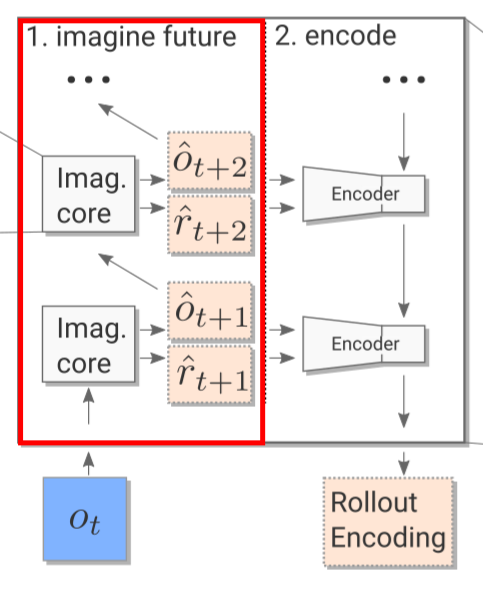
\includegraphics[height=.5\textheight]{./Images/imagine_future.png}%
	\end{center}
\end{multicols}
    
\end{frame}
\clearpage

%%%%%%%%%%%%%%%%%%%%%%%%%%%%%%%%%%%%%%%%
%% Folie: Bilder - Zweispaltige Seite %%
%%%%%%%%%%%%%%%%%%%%%%%%%%%%%%%%%%%%%%%%
\begin{frame}
    \frametitle{I2A Architecture - Encoder}

\begin{multicols}{2}
	\begin{PraesentationAufzaehlung}
		\item CNN Network followed by an LSTM Network
		\item CNN Network:\\
		Encode observation and reward $\hat{o}_{t+i}, \hat{r}_{t+i}$
		\item LSTM Network:\\
		Learns long-term dependencies
		%\item Learns useful information from the rollout trajectories
	\end{PraesentationAufzaehlung}
    \vfill\columnbreak
	\begin{center}
    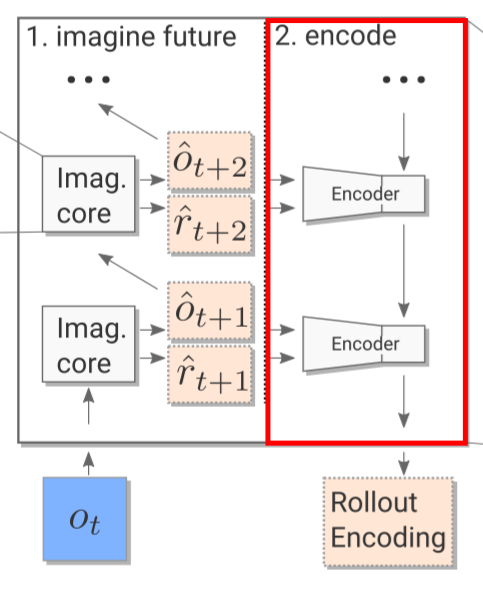
\includegraphics[height=.5\textheight]{./Images/encoder.png}%
	\end{center}
\end{multicols}
    
\end{frame}
\clearpage


%%%%%%%%%%%%%%%%%%%%%%%%%%%%%%%%%%%%%%%%
%% Folie: Bilder - Zweispaltige Seite %%
%%%%%%%%%%%%%%%%%%%%%%%%%%%%%%%%%%%%%%%%
%\begin{frame}
%    \frametitle{I2A Architecture - Model Free Path}

%\begin{multicols}{2}
%	\begin{PraesentationAufzaehlung}
%		\item 
%	\end{PraesentationAufzaehlung}
%    \vfill\columnbreak
%	\begin{center}
%    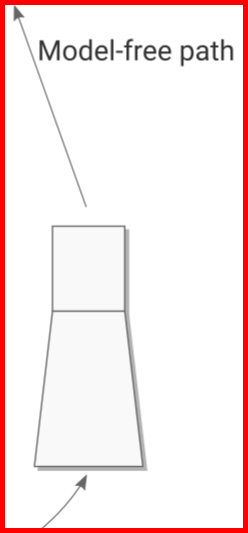
\includegraphics[height=.5\textheight]{./Images/i2a_model_free_path.png}%
%	\end{center}
%\end{multicols}
%    
%\end{frame}
%\clearpage


%%%%%%%%%%%%%%%%%%%%%%%%%%%%%%%%%%%%%%%%
%% Folie: Bilder                      %%
%%%%%%%%%%%%%%%%%%%%%%%%%%%%%%%%%%%%%%%%
\begin{frame}
    \frametitle{I2A Architecture - Model Based Path}


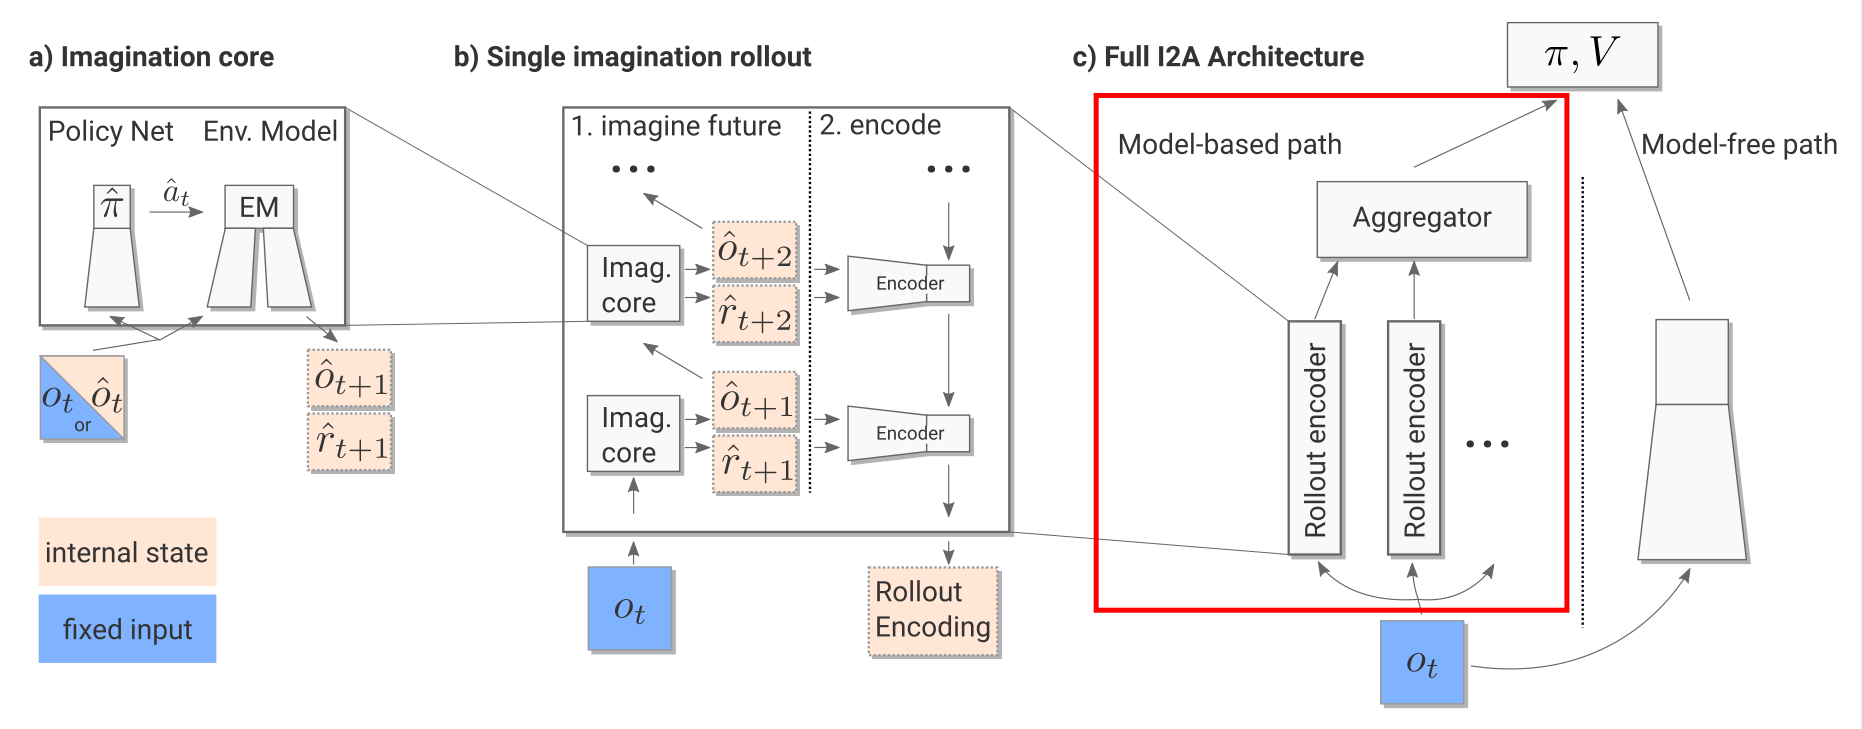
\includegraphics[width=\columnwidth]{./Images/i2a_all_model_based_path.png}%

%For each action $a$ the agent can take do a imagination rollout 
% the future based on a model of the environment and use this information for decision making
    
\end{frame}
\clearpage

%%%%%%%%%%%%%%%%%%%%%%%%%%%%%%%%%%%%%%%%
%% Folie: Bilder - Zweispaltige Seite %%
%%%%%%%%%%%%%%%%%%%%%%%%%%%%%%%%%%%%%%%%
\begin{frame}
    \frametitle{I2A Architecture - Model Based Path}

\begin{multicols}{2}
	\begin{PraesentationAufzaehlung}
	    \item For each action $a$ the agent can take, do a imagination rollout 
		%For each action the agent can take, 
		%imagine the future% and learn relevent information that can happen
		\item Aggregator: \\
		Concatinate all action rollouts
	\end{PraesentationAufzaehlung}
    \vfill\columnbreak
	\begin{center}
    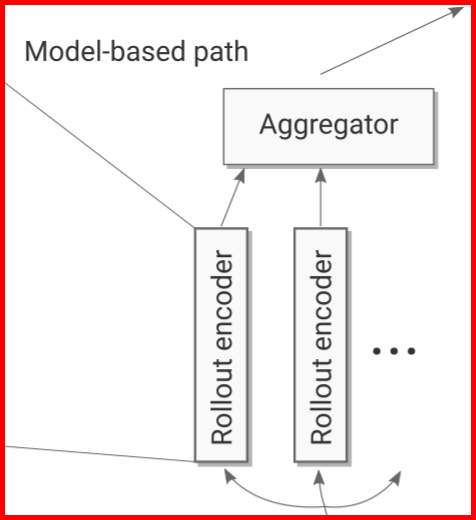
\includegraphics[height=.5\textheight]{./Images/i2a_model_based.png}%
	\end{center}
\end{multicols}
    
\end{frame}
\clearpage




%%%%%%%%%%%%%%%%%%%%%%%%%%%%%%%%%%%%%%%%
%% Folie: Bilder                      %%
%%%%%%%%%%%%%%%%%%%%%%%%%%%%%%%%%%%%%%%%
\begin{frame}
    \frametitle{I2A Architecture - Model Free Path}


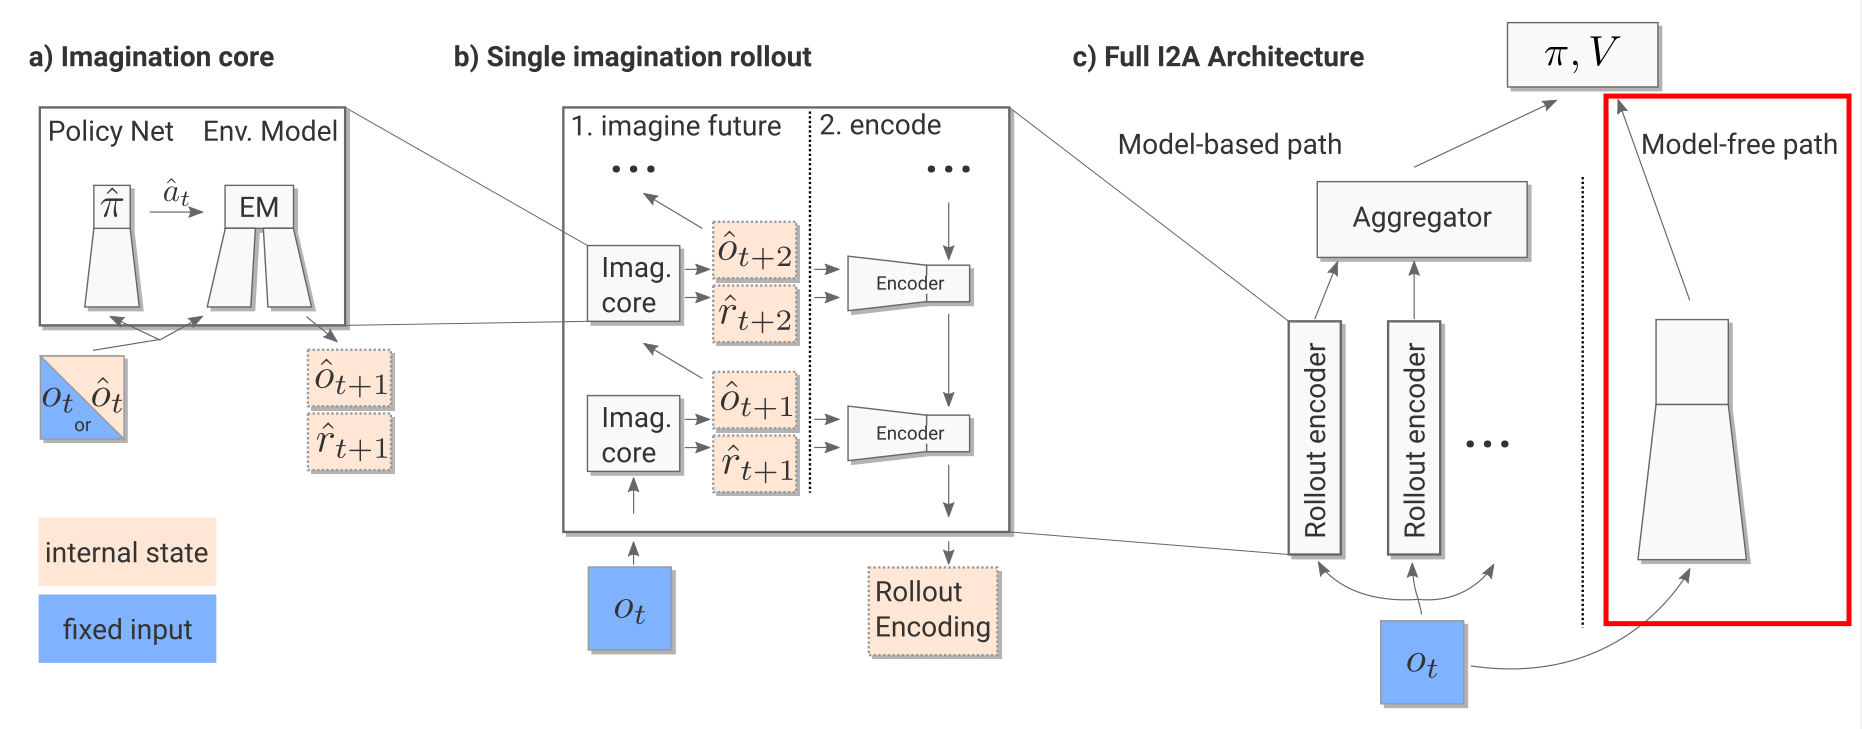
\includegraphics[width=\columnwidth]{./Images/i2a_all_model_free_path.png}%

\begin{PraesentationAufzaehlung}
	\item CNN Layers followed by Fully Connected Layers
\end{PraesentationAufzaehlung}

\end{frame}
\clearpage



%%%%%%%%%%%%%%%%%%%%%%%%%%%%%%%%%%%%%%%%
%% Folie: Bilder - Zweispaltige Seite %%
%%%%%%%%%%%%%%%%%%%%%%%%%%%%%%%%%%%%%%%%
\begin{frame}
    \frametitle{I2A Training}

\begin{multicols}{2}
	\begin{PraesentationAufzaehlung}
		\item Input:\\
		Observation $o_t$
		\item Output:\\
		Policy $\pi$ and value function $V$
		\item Train with Advantage-Actor-Critic (A2C)
	\end{PraesentationAufzaehlung}
    \vfill\columnbreak
	\begin{center}
    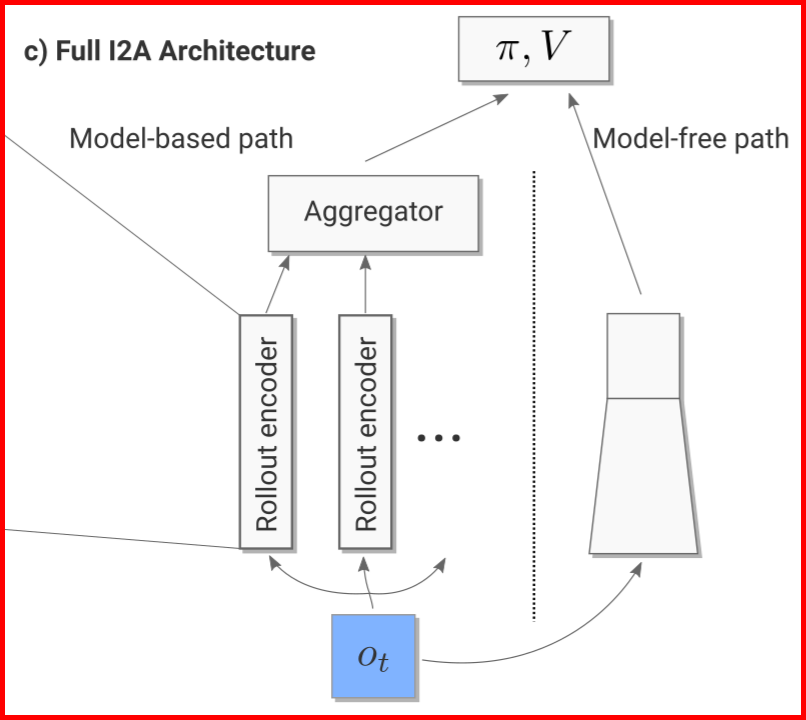
\includegraphics[width=\columnwidth]{./Images/i2a_a2c.png}%
	\end{center}
\end{multicols}
    
\end{frame}
\clearpage






%%%%%%%%%%%%%%%%%%%%%%%%%%%%%%%%%%%%%%%%%%%%%%%%%%%%%  
 % FOLIENSTIL: Weisse Schrift auf blauem Grund 
\PraesentationMasterWeissBlau 
\begin{frame} 
    \frametitle{MiniPacman}
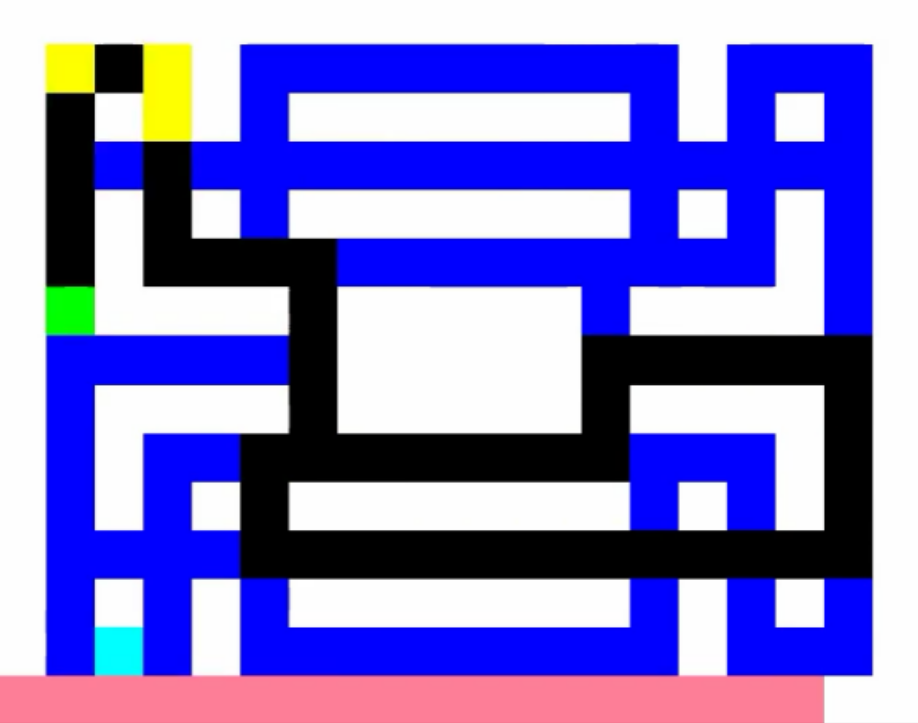
\includegraphics[height=0.5\textheight]{./Images/mini_pacman.png}%
\end{frame} 

\PraesentationMasterStandard

%%%%%%%%%%%%%%%%%%%%%%%%%%%%%%%%%%%%%%%%
%% Folie: Bilder - Zweispaltige Seite %%
%%%%%%%%%%%%%%%%%%%%%%%%%%%%%%%%%%%%%%%%
\begin{frame}
    \frametitle{MiniPacman}

\begin{PraesentationAufzaehlung}
	\item I2A Model Based Path expensive to train
	\item Uses 15 x 19 Grid World version of Pacman
	\item Makes vision problem easier but preserves the reinforcement learning problem
	\item MiniPacman can be played in different modes
\end{PraesentationAufzaehlung}
    
\end{frame}
\clearpage

%%%%%%%%%%%%%%%%%%%%%%%%%%%%%%%%%%%%%%%%
%% Folie: Bilder - Zweispaltige Seite %%
%%%%%%%%%%%%%%%%%%%%%%%%%%%%%%%%%%%%%%%%
\begin{frame}
    \frametitle{MiniPacman -- Hunt}

Rewards:

	\hspace{-4mm}
	\begin{tabular}{ p{7cm}  r }
 	At each step & 0 \\
  	Eating food & 0 \\
	Eating power pill & 1\\
	Eating ghost & 10\\
	Killed by ghost & -20\\
	\end{tabular}
    
\end{frame}
\clearpage


%%%%%%%%%%%%%%%%%%%%%%%%%%%%%%%%%%%%%%%%
%% Folie: Bilder - Zweispaltige Seite %%
%%%%%%%%%%%%%%%%%%%%%%%%%%%%%%%%%%%%%%%%
\begin{frame}
    \frametitle{EnvironmentModel Hunt Demo}
    
\end{frame}
\clearpage




%%%%%%%%%%%%%%%%%%%%%%%%%%%%%%%%%%%%%%%%
%% Folie: Bilder - Zweispaltige Seite %%
%%%%%%%%%%%%%%%%%%%%%%%%%%%%%%%%%%%%%%%%
\begin{frame}
    \frametitle{I2A MiniPacman Hunt Results}

\begin{multicols}{2}
	\begin{center}
    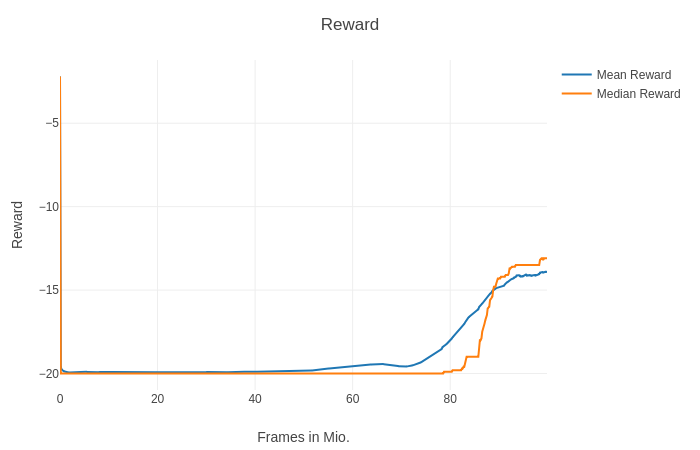
\includegraphics[width=\columnwidth]{./Images/a2c_hunt_reward.png}\\
	A2C Hunt Reward Training Curve (100 mio frames)
	\end{center}
    \vfill\columnbreak
	\begin{center}
    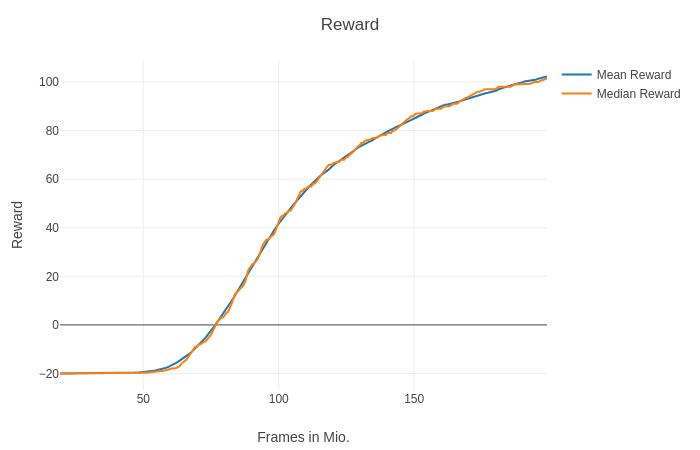
\includegraphics[width=\columnwidth]{./Images/i2a_hunt_reward_mean_and_median.png}\\
	I2A Hunt Reward Training Curve (200 mio frames)
	\end{center}
\end{multicols}
\end{frame}
\clearpage

%%%%%%%%%%%%%%%%%%%%%%%%%%%%%%%%%%%%%%%%
%% Folie: Bilder - Zweispaltige Seite %%
%%%%%%%%%%%%%%%%%%%%%%%%%%%%%%%%%%%%%%%%
\begin{frame}
    \frametitle{I2A Hunt Demo}
    
\end{frame}
\clearpage

%%%%%%%%%%%%%%%%%%%%%%%%%%%%%%%%%%%%%%%%
%% Folie: Bilder - Zweispaltige Seite %%
%%%%%%%%%%%%%%%%%%%%%%%%%%%%%%%%%%%%%%%%
\begin{frame}
    \frametitle{Final Conclution}

\begin{PraesentationAufzaehlung}
	\item Working Environment Model and I2A implementation
	\item Based on A2C implementation of Kostrikov \url{https://github.com/ikostrikov/pytorch-a2c-ppo-acktr} 
	\item Will be published on github
\end{PraesentationAufzaehlung}
    
\end{frame}
\clearpage


%%%%%%%%%%%%%%%%%%%%%%%%%%%%%%%%%%%%%%%%
%% Folie: Bilder - Zweispaltige Seite %%
%%%%%%%%%%%%%%%%%%%%%%%%%%%%%%%%%%%%%%%%
\begin{frame}
    \frametitle{Thank you for your attention! \vspace{15mm}
	 \\Questions?}
    
\end{frame}
\clearpage



